\section{UI Gesture Collection}
\subsection{Introduction}

Multitouch gestural interfaces, like those found on tablets and smartphones, offer the possibility of a very direct user experience, especially compared to the Windows, Icons, Mouse, Pointer (WIMP) interface design. 
Rather than, for example, using an arrow key to scroll in a document, the user can drag the document directly, as though they were sliding a long piece of paper on a table. 

This directness is a hallmark of what has come to be called Natural User Interfaces, or NUI. 
A natural user interface is one that allows the user to re-use existing skills and natural motions to interact directly with content \citep{blakeNUIWin}. 
In practice, this means that the elements of the interaction are actions such as pointing and other gestures, drawing with a pen, speech, gaze, and so forth, rather than computer-specific interface devices. 
By way of contrast, the command line interface is defined in terms of typing with some form of keyboard, and the graphic user interface is (in most cases), defined in terms of mouse actions. 

However, as the number of operations the user wishes to perform increases, the limitations of multitouch screens become more apparent. 
Screens are flat, and so only afford 2-dimensional gestures, such as dragging, poking, and tapping. 
Even if the screen depicts a 2-dimensional projection of a 3-dimensional world, operations that would make sense in the 3D world, such as grasping, have to be mapped to the 2-dimensional space of operations to be performed. 
Typically, the gestures that the user uses to perform the available operations are chosen by the interface developer, and the user is trained to perform them, possibly by a short tutorial program \citep{wobbrock2009user, vanacken2008ghosts, freeman2009shadowguides}. 

Unfortunately, the use of screens with interactions inspired by the affordances of physical objects leads to the user having to decide between ``natural'' skills and motions, which are used on physical objects, and the skills and actions used with screens: single-point dragging and clicking. 
Most users understand that they are looking at pictures of things on a screen, and so default to single-point interactions \citep{vanacken2008ghosts}.

However, the behavior of users interacting with an NUI device is not solely informed by their intuitions about the physical objects represented on the screen. 
Smartphones, tablets, and other multitouch user interface devices, as well as specific types of computer programs, such as CAD and realtime strategy game programs, also inform the user's expectations about interactions with new interfaces. 
Rather than claiming that the users are untrained, and the gestures are ``intuitive'', it would be more accurate to claim that the users already have a form of training, from the devices that they use in their daily lives. 
In this paper, we attempt to discover the gestures that users would choose themselves, based on their own thinking about the interface and their own past experience with computer technology such as tablets, smartphones, and video games. 

This work is an extension of previous work that used a similar process to discover user interface gestures for single or small groups of robots \citep{Micire:2009:ANG:1731903.1731912}. We extend this method to larger groups of robots, in an attempt to discover if the gestures that users select vary with the number of robots available.

More specifically, it is hypothesized that there exists a swarm size beyond which users will transition from treating the swarm robots as individuals to interacting with the robots in small groups or as a single large group. 
This transition point will be apparent because of a change in the gesture set that users choose to interact with the swarm. 
Rather than issuing one command for each robot, the user will instead use commands that control the bulk of the robots as a cloud or flock, but may leave some robots unused. 
For example, the user may switch from selecting robots as individuals to shaping the group as if sculpting, with pushing and pinching to ``carry'' groups around. 
The user may also change how they indicate which robots are to be interacted with. 
Rather than selecting each robot by clicking on it, the user might circle a group they want to use, or simply assume that the same command is issued to all robots by default. 
The size of the swarm where changes in the user gestures occur will indicate the transition point between the user intending to interact with individual robots as opposed to interacting with the swarm as a whole. 

Further, it is hypothesized that altering how the user interface displays the location of the robots in the swarm will affect the transition point.
Once the ratio of the size of individual swarm members to the size of the area the swarm is in becomes sufficiently small, displaying the swarm members at the same scale as the map will result in the representation of the swarm members being too small to interact with. 
Scaling the representation of the robots up, relative to the map, could make the robot representations overlap unrealistically and obscure the map. 
Instead, we propose that for certain scales of swarms, it makes sense to represent the swarm as the area covered by the swarm, rather than the locations of the individual robots.
This approach has been used successfully for navigation in three dimensions, by developing a controller that causes the individual UAVs to remain within a bounding prism, and allowing the user to control the shape and location of that prism, instead of the location of each individual UAV \citep{ayanian2014controlling}.
 
More specifically, a display which obscures individual robots and displays a cloud or swarm boundary will cause the user to treat the swarm as a whole rather than individuals, which will be apparent because the user will use the same gestures that users select for controlling individual robots. 

\subsection{Related Work}

Previous attempts to build user interface gesture sets can be broadly separated into two classes: those that attempt to build a general gesture set, and those that attempt to build a gesture set to be used for a specific task. 

General gesture sets would be for operations such as the cut/copy/paste editing metaphors, which show up in word processing, image editing, and other productivity applications. 
These operations act in related but differing ways, depending on their context, but are invoked in the same way across applications and even across operating systems. 

Wobbrock, Morris, and Wilson use an interesting technique to elicit general user-interface gestures from non-technical users \citep{wobbrock2009user}.
The user is shown the \textit{effect} of a command, and then asked to perform the gesture that \textit{caused} that effect. 
The users were asked to think aloud, in order to understand their cognition about the system and gestures, in addition to their behaviour. 
The experiment used 27 commands: move a little, move a lot, select single, rotate, shrink, delete, enlarge, pan, close, zoom in, zoom out, select group, open, duplicate, previous, next, insert, maximize, paste, minimize, cut, accept, reject, access menu, help, task switch, and undo (listed in order of complexity as ranked by Wobbrock \textit{et al}).
Many of these commands are related to window managers, or occur in some form in multiple applications, such as the cut/copy/paste metaphors.

Task-specific gestures are for operations such as flying through a 3D rendering of an architectural space, or transposing cells in a spreadsheet. 
While somewhat intuitive gestures may exist for both operations, the operation is tightly bound to the task at hand, and the gestures would likely be different. 

Yao, Fernando, and Wang develop a set of task-specific gestures for urban planning from the required functionality of the interface and paper prototyping on a table \citep{yao2012multi}. 
The gestures were collected by placing a map on the table, and asking users to perform the gestures they would use to access the required functions. 
The resulting interface is modal, depending on the user's desired method of interaction, different gestures are available. 
The interface also permits the combination of some gestures, such as panning or rotating the map while zooming in or out as well. 

Micire \textit{et al}. develops a taxonomy of user gestures for control of both robots and of the interface to control them \citep{Micire:2009:ANG:1731903.1731912}. 
The interface control gestures are for actions such as zooming in on the content of the screen or panning around a map. 
Individual users chose a variety of gestures to perform the tasks, but for almost all types of tasks, having two gestures available to perform it would be sufficient to cover 60\% of the users. 
It was also noted that the gestures that users use are informed by their previous experience both with WIMP interfaces and with touch-screen technology. 
Since smartphones are a common multitouch interaction device, it would be expected that smartphone users expectations of multitouch interaction would be informed by their phones. 
Micire \textit{et al}. confirmed this, finding that iPhone owners used significantly more pinch gestures than participants with no iPhone experience. 
 
As a result, this general gesture set could be used in a gestural window manager or operating system interface, while the gesture sets developed by Micire \textit{et al}; Yao, Fernando, and Wang; or in this work are all intended to provide a more precise set of meanings for a single application and task. 

\subsection{Experiment Setup}

\todo{put a picture of the experiment setup here}


Users were seated in front of the interface and read a script describing the system and the experiment. The user interface displayed alternating slides of instructions to the user, such as ``Move the robots to area A", and interface screens for them to interact with. 
The interface did not visibly respond to user contact or move the robots depicted on it.
In this regard, it more closely resembles the paper prototypes of the User-Centered Design process than a fully functional interface \citep{ehn1992cardboard}.

The multitouch user interface device used in this experiment is a 3M M2265PW touchscreen. 
This screen can track up to 20 simultaneous points, but reports only points, rather than shapes or areas of contact. 
While the user interacted with the touch screen, their touches and the positions of their hands were recorded by the computer connected to the screen and by the video cameras. 
One video camera was placed high, looking down at the screen, to track where the user's hand position over the screen. 
The other video camera was placed in front of the screen at a low angle, in order to observe whether the user's hands were touching the screen, or moving above it. 
In addition to screen contacts and video, users were asked to think aloud about their actions.
A microphone placed near the screen was used to record everything the user said. 

The software used to record all of this information is ROS, the Robot Operating System \citep{ROS_announcement_paper}. 
ROS was developed as a message-passing framework and hardware abstraction layer for robots. 
Software using ROS is implemented as ``nodes'', which communicate by passing messages, generally in a publisher/subscriber pattern. 
The format of the messages is formally defined, and the generation of the code for generating messages and handling routing of messages is provided by ROS. 

It may seem unusual to use a framework intended for operating robots as a recording program for collecting experiment data, but ROS provides a utility called rosbag that records some or all of the messages emitted by the robot's sensors in a ``bag'' file. 
In this case, the cameras, microphone, and UI application are the ``sensors'' which rosbag records.
A ROS launch file starts multiple ROS nodes to record image data from the cameras, audio from the microphone, and touch events and screen updates from the UI.
ROS also provides tools for manipulating bag files, and playing them back. 
All of the data in the file is timestamped, so it plays back with the audio, video, and UI interactions all accurately synchronized. 
Because all of the data is treated as standard ROS message types, it is relatively easy to write custom processors for the recorded data.
For example, a node was written that accepts the replayed UI screen changes and touch events, and renders them as a stream of ROS image messages showing the contact points overlaid on the UI screen. 

\subsubsection{Experiment Conditions}

Users were given tasks in one of five conditions, varying by how many robots were in each condition. 
The conditions consisted of 1-2 robots, 10 robots, 100 robots, 1000 robots, or an unknown number of robots, represented by a cloud. 
For each condition, the user was requested to perform a sequence of tasks. 
The exact number of tasks varied between conditions due to some tasks not making sense with the number of robots involved. 

\begin{tabular}{l|l|l|l|l|l}
& 1 & 10 & 100 & 1000 & Unknown \\
Move to area A & x & x & x & x & x\\
Move to area A with a wall & x & x & x & x & x \\
Stop the robots & x & x & x & x & x\\
Divide around an obstacle & & x & x & x & x \\
Orange to B, red to A & x & x & x & x & x \\
Orange to A, red to B & x & x & x & x & x \\
Orange to A, red to B (mixed) & x & x & x & x & x \\
Divide group & x & x & x & x & x \\
Merge groups & & x & x & x & x \\
Form a line & & x & x & x & x \\
Form a square & & x & x & x & x \\
Move the crate to area A & x & x & x & x & x \\
Move the crate to area A (dispersed) & x & x & x & x & x\\
Mark defective robot & x & x & x & x & \\
Remove defective robot & x & x & x & x &  \\
Patrol the screen border & x & x & x & x & x \\
Patrol area A & x & x & x & x & x \\
Disperse over screen & x & x & x & x & x \\
\end{tabular}

The individual robot case is lacking the tasks that do not make sense for a single robot. A single robot cannot, for example, divide around an obstacle or form a square. 
The ``Merge groups" task was left out of the single robot case because of the potential for confusion when referring to a single robot as a group. 

The unknown number of robots condition has the same tasks as the 10, 100, and 1000 robot cases, except for the ``Mark defective robot" and ``Remove defective robot" task. 
Without UI elements that represent individual robots, the user cannot take any actions that refer to a specific robot. 

\subsection{Analysis}

User gestures were coded using a methodology adopted from the social sciences, Grounded Theory \todo{cite}.
Grounded Theory is an iterative process, where the data are first coded at a very fine-grained level, and then the resulting coded elements are compared to each other to try to determine their qualities, similarities, and differences. 
Codes can be consolidated or divided until repeated passes of coding and comparison no longer alter the emerging structure of the coding scheme. 
During each iteration of coding and comparison, the coder makes memos as well, describing the links they see between related coded elements and higher-level abstractions that relate the elements. 
These memos are eventually written up as the social scientific theory, which is believed to be grounded in the data because it arises from the coding process. 

\subsubsection{Initial coding pass}

The inital pass used open coding, where the ``codes'' were essentially free-form text entry. 
Rough counts of the open codes for the first 10 participants indicated that ten of the codes covered 81\% of the 580 total coded events. 
The ten most heavily used codes are, in order of occurrence: drag, tap, voice command, box select, 2 finger drag, double-tap, lasso, tap and hold, 2 handed drag, reverse pinch, and parallel hands. 
This pass of coding indicated that a majority of the user actions could be coded as some form of drag, some form of tap, box or lasso selection, pinch, and parallel hands. 

The most common code was drag, which accounts for 37.58\% of the rough coding, or 42.07\% if all forms of drag in the top ten codes are considered. ``Drag'' is when the user places one finger down, moves it to another location, and raises it again. Two finger drag is the same, only with two fingers on the same hand placed on the screen rather than one. Two-handed drag is single-finger drag, but executed with both hands at the same time. 

The second most common code was ``tap'', with 20.34\% of the rough coding, or 25.34\% if tap, doubletap, and tap and hold are all considered. Tap is when the user places a finger down and then very quickly raises it again. Double-tap is two taps in the same location in quick succession. Tap and hold is when the user places their finger on the screen and leaves it in one place for more than a second before raising it. 

Box select consists of a diagonal (relative to the screen edges) drag gesture over the robots or another object on screen, with the intent to select everything within the box whose diagonal is represented by the drag. 
Lasso select is a drag which ends near where it began, forming a loop, with the intent to select everything inside the loop. 

Pinch and reverse pinch are essentially two-hand drag or two-fingered drag but with the hands or fingers moving towards (pinch) or away (reverse pinch) from each other.
This gesture is common for zooming in multitouch user interfaces on smartphones. 

Voice command was used to code when a user spoke a command out loud, rather than using gestures. The high incidence of voice commands (7.07\% of all codes) in the first ten users can be attributed to a single user who issued commands almost exclusively through voice. 

The final gesture, ``parallel hands'' is placement of the hands, palms facing each other, over some area of the screen. This gesture was used many times by the same user who issued voice commands, to indicate where the robots should form a line. Because parallel hands only accounted for 0.69\% of the gestures, it was left out of the development of the coding application for the second stage of coding. 


 
\subsubsection{Second coding pass}

To facilitate coding in the second pass, an application was developed to record codes. 
The application has coding functions for the six most common gestures: drag, tap, voice command, box select, lasso select, and pinch. 
It also includes coding functions for user interface elements described by the user, such as buttons or menus, a function to code user gestures not covered by the six most common gestures, and a function for coders to enter free-form text memos. 

\todo{Need to make the call as to whether example gestures that users made should be counted along with ``real'' gestures, or left out. Maybe go both ways and see if it affects anything.}

A second pass of coding of the first ten user recordings was performed by two coders. 

Because the coders were responsible for deciding which user actions to code, as well as how to code them, it is possible for one coder to miss a gesture that another coder codes, or to split a single gesture into two coded units instead of one. 
For example, one coder initially split spoken commands at conjunctions such as "and", resulting in two units both coded as voice commands, while the other coder coded the entire sentence as a single unit. 
This leads to the possibility that for a single task, the coders will produce different length lists of coded units. 
Cohen's kappa is a measure of inter-coder reliaibility for categorical items, but it assumes that both coders are coding the same number of codable units \citep{cohen1960coefficient}. 
It does not account for the possibility of missing data. 
Extending Cohen's kappa by adding a null code for absent data leads to artificial inflation of the inter-coder reliability, so this approach was rejected.
Cohen's kappa is also influenced by the true prevalence of a code in the set of codable units, which is to say that coding data which actually contains a large number of occurrences of one code can artificially inflate Cohen's kappa. 
The ``drag'' gesture is by far the most common gesture used [put prevelence here] \todo{how much effect would that have on k?}


Krippendorf's alpha permits data to be absent \citep{hayes2007answering}. 
To calculate Krippendorf's Alpha for the coded events during a task, each event from one coder was matched with the event chronologically closest to it produced by the other coder.
Any remaining events were assumed to have been spotted by one coder, but missed by the other, resulting in missing data. 
Krippendorf's alpha was then calculated on the resulting list of pairs of coded events, with each pair being assumed to represent the same coding unit. 

[Put some proper info on the attained alphas here]



[DATA INTENSIFIES]
 
Some people \todo{how many people?} take the directions on the slides very literally. 
For example, users who had been solely using the touch interface read the slides that instructed ``Tell the robots to form a line" to indicate that they should speak the words ``Form a line", addressed to the robots.

People \todo{how many people?} who didn't otherwise want voice commands would use them for the task of stopping the robots. 
Since this task assumes the robots are already moving towards a goal, attempts to interact with all of them while they are moving could be difficult. 

For the task of removing the defective robot, the location selected for it to be removed to was usually either a corner, a ``recycle bin" or similar disposal area, or off the edge of the screen. This use of the area beyond the screen for placement of deleted or rejected things parallels that seen by Wobbrock \textit{et al}.

\subsubsection{Robot Count in Unknown Number Case}

In the condition where the exact number of robots was unknown, and the swarm was depicted as a cloud, participants were asked to say how many robots they felt the cloud represented. 
Generally, the participant expectation was that the cloud represented tens of robots, but simply averaging the responses would not be useful, as one participant said that it ``could be millions''. 
For those that did answer with a single number or range, the answers were 10-20, 10-``hundreds'', 12, 7, 10, 2-10, 10-12, 2-``millions', 5-10, 8, and 50. 
If the endpoints of ranges are treated as answers, with ``hundreds'' and ``millions'' set to 500 and 5,000,000 respectively, the median answer is 10, but the mean and standard deviation are not illustrative of the user responses. 
Rejecting ``hundreds'' and ``millions'' as outliers gives a mean of 11.86, with a standard deviation of 11.04, which adequately covers the common intuition that the swarm contains at least 2 members and many have tens, but not likely hundreds, of robots in it.

Participant comments may shed some light on the source of this intuition. 
One participant indicated during the study that they interpreted the corners of the polygonal cloud as possible robot locations, and so drew an idea of the scale of the swarm from the number of corners. 
The cloud has 11 corners, 7 convex and 4 concave, which is consistent with the estimated robot count. 

Another participant said their estimate was informed by the instructional slides preceding the test, which depicted a number of robots, the outline around them, and the resulting cloud, as shown in fig. \ref{instructional_slides}. 
These slides depicted 10 robots, and so may have biased participants to expect that the cloud had 10 robots in it. 
However, multiple participants stated that the cloud represented an unknown number, or estimated more or less than 10 robots.

\begin{figure}
	\centering
	\begin{subfigure}{0.3\textwidth}
		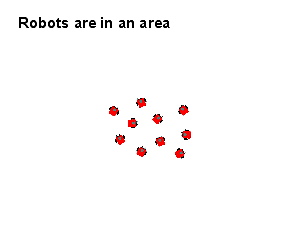
\includegraphics[width=\linewidth]{../ui_experiment/slide_images/Swarm_Robot_Control_-_Unknown_Number_of_Robots_0001.png}
	\end{subfigure}
	\begin{subfigure}{0.3\textwidth}
		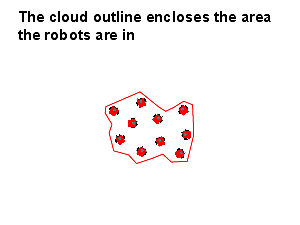
\includegraphics[width=\linewidth]{../ui_experiment/slide_images/Swarm_Robot_Control_-_Unknown_Number_of_Robots_0002.png}
	\end{subfigure}
	\begin{subfigure}{0.3\textwidth}
		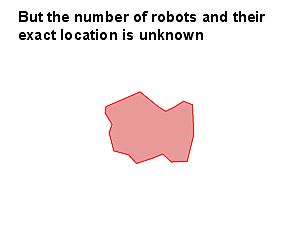
\includegraphics[width=\linewidth]{../ui_experiment/slide_images/Swarm_Robot_Control_-_Unknown_Number_of_Robots_0003.png}
	\end{subfigure}
	\caption{Instructional slides for the unknown number of robots condition, showing cloud representation of robot swarm.}
	\label{instructional_slides}
\end{figure}

\subsubsection{Selection Strategy}

At the end of the experiment, users were shown an image of a robot swarm, with a dotted line around it depicting a finger drag path around some of the robots. 
The users were told that the intent of this gesture was to select robots, and asked to indicate which robots in the image were selected, or in the unknown number of robots case, whether the gesture selected all of the robots or left any out. 
Users in the single robot case were shown the selection image with ten robots in it, because the with one robot, there are not enough robots to have a selection which may exclude some robots and include others. 

\begin{figure}
	\centering
	\begin{subfigure}{0.48\textwidth}
		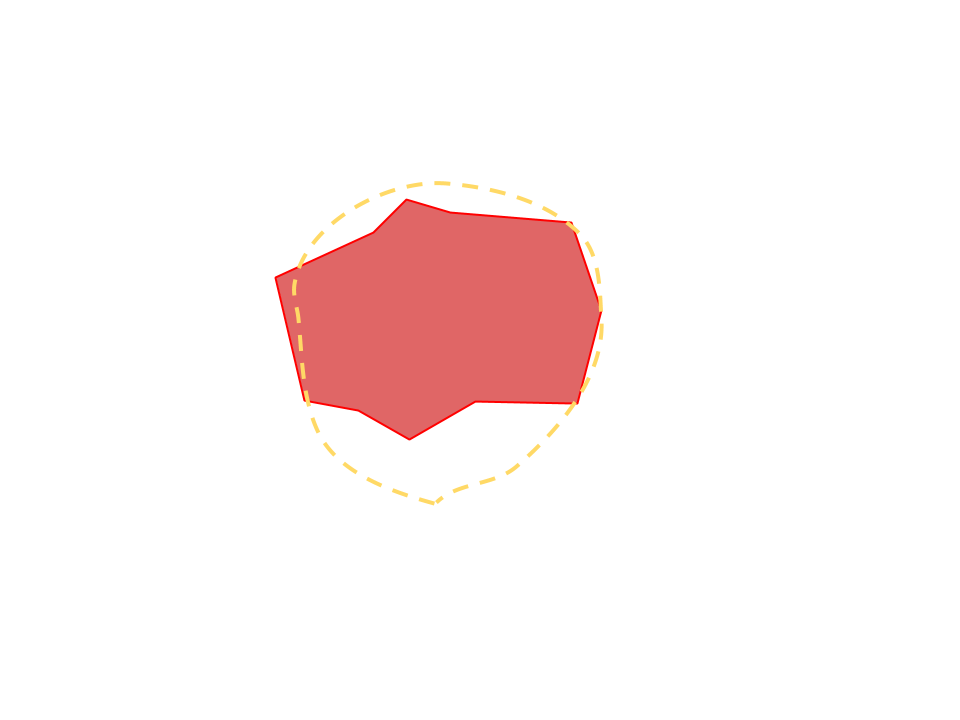
\includegraphics[width=\linewidth]{../Selection_Fuzz_X.png}
	\end{subfigure}
	\begin{subfigure}{0.48\textwidth}
		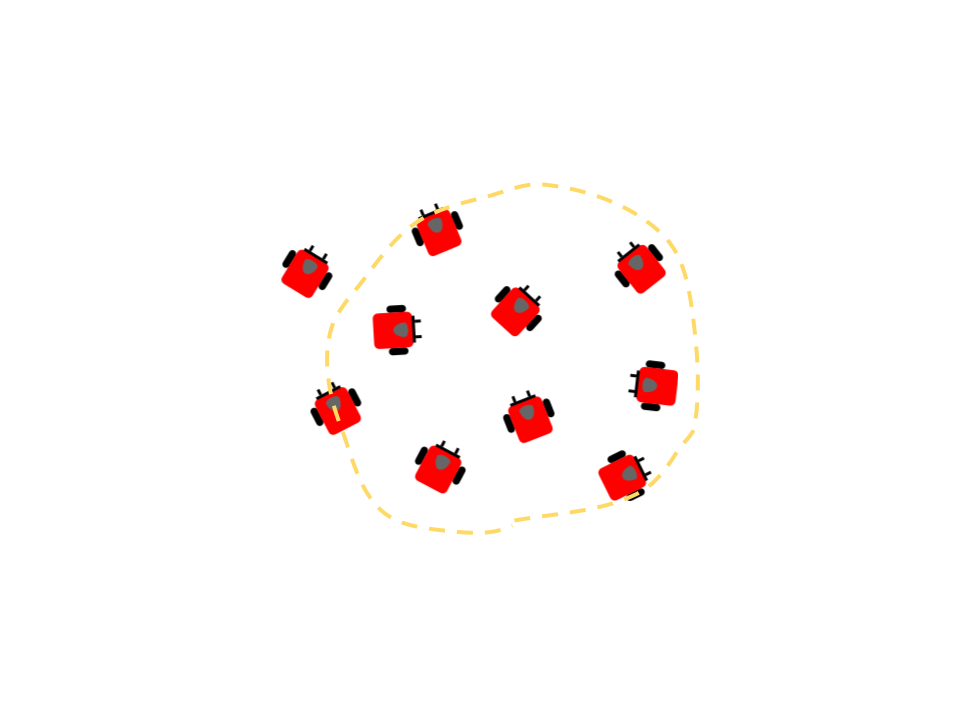
\includegraphics[width=\linewidth]{../Selection_Fuzz_10.png}
	\end{subfigure}
	\begin{subfigure}{0.48\textwidth}
		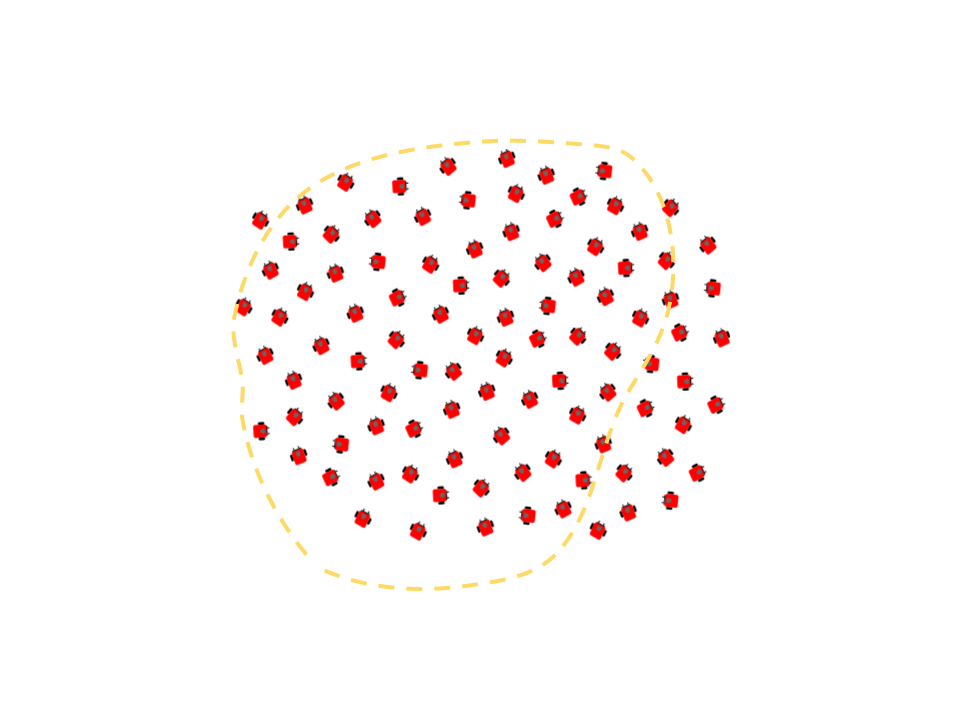
\includegraphics[width=\linewidth]{../Selection_Fuzz_100.png}
	\end{subfigure}
 	\begin{subfigure}{0.48\textwidth}
		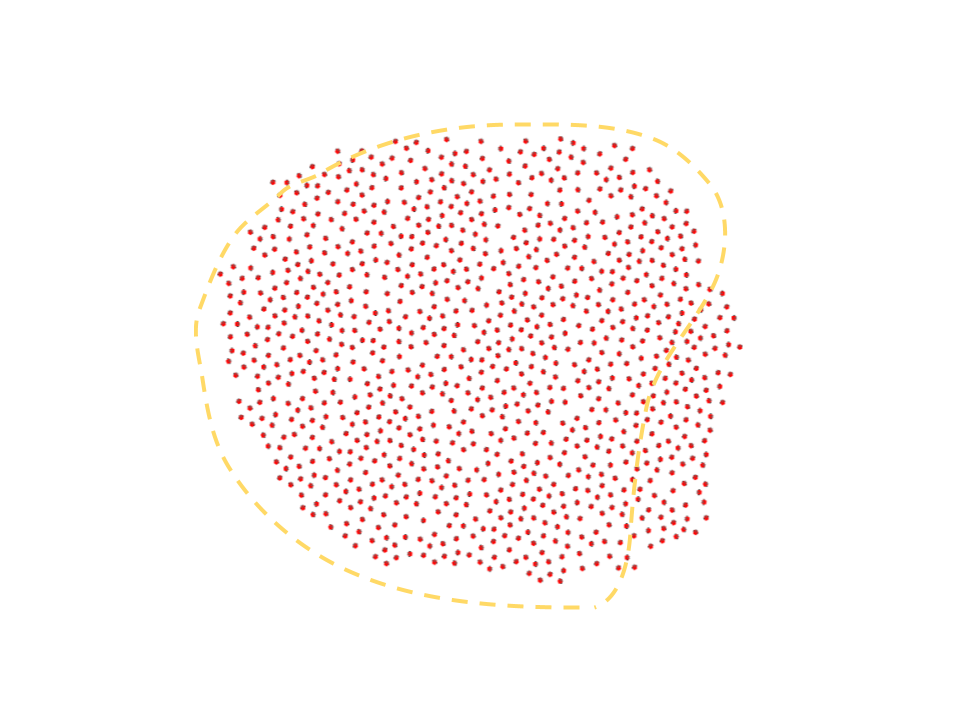
\includegraphics[width=\linewidth]{../Selection_Fuzz_1000.png}
	\end{subfigure}
		\caption{Images for selection strategy question.}
	\label{strategy_question}
\end{figure}

In the unknown number of robots case, 7 participants indicated that all the robots were selected, 3 of the participants indicated that some robots were left out, and one participant indicated that whether the selection included all of the robots could depend on the task. 

Because the 1 and 10 robot cases saw the same selection image, they are reported together. 
12 participants indicated that robots that were inside the selection or touched by the selection line should be considered selected. 
2 participants indicated that robots depicted with half or more of the robot inside the circle should be considered selected. 
One participant indicated that the robot half out of the circle should \emph{not} be selected. 
One participant indicated that robots on the border should be included or not included in the selection, depending on the task. \todo{Three answers are missing, find those and fix}
One user indicated that only the first robot touched should be selected, which is consistent with control strategies that move each robot individually. 

For the hundred robot case, 3 participants indicated that robots inside or touching the line were selected. 
3 participants said that robots should be mostly inside the line to be counted, with one participant stating that robots should be 80\% or more inside the line to count. 
2 participants indicated that robots should be more than halfway inside the line to be selected. 
One participant stated that only robots completely inside the line should be counted. \todo{One answer missing, find and fix}
 
In the thousand robot case, 7 participants indicated that robots inside or touching the line should be selected. 
2 participants indicated that robots must be completely inside the line to be selected. 
1 participant indicated that robots mostly inside the line should be selected. 

Overall, participants generally err on the side of inclusion, rather than exclusion of robots from selection.
If a user interface is required to include or exclude ambiguous elements from a selection, it appears that including ambiguous elements will satisfy users. 
User comments also suggested that ways to amend selections before further commanding the robots would be desirable. \todo{was there any consistency in \emph{how} to do this} 

 \begin{tabular}{ l l l l l}
   Condition & Completely inside & Half or more in & Touching line & Other\\
   \hline
   10 & 0 & 2 & 12 & 3 \\
   
   100 & 1 & 5 & 3 & 0 \\
   1000 & 2 & 1 & 7 & 0\\
   \hline
   Totals & 3 & 8 & 22 & 2 \\
 \end{tabular}

%It is interesting to note that two participants, one from the unknown number of robots case, and one from the 10 robot case, said that in cases of ambiguous selection, the system should add or remove robots from the selection based on the task. 
%As the system cannot predict the task it is about to be commanded to perform, it is likely best to err on the side of selecting too many robots, rather than too few. 

\todo{go over metaphor failure in NUI. People know things are just pictures, so we get things like moving the wall to stop the robots (in the real world, mobile walls are rare).}

\todo{Wobbrock et. al. style would have been a better way to structure this experiment. Some users were initially confused with the interface not responding, so showing the response, and then asking for the gesture may have been a better idea. Some users also didn't try to do the task (no color sorting) or got it wrong (no cross-over in crossover condition.) Showing the response may have prompted that better. }

\subsubsection{Participant Demographics}

The experiment had 51 participants, 11 in the unknown number of robots condition and 10 in all other conditions. 29 of the participants were male, 22 were female. The average age of participants was 22.1 years, with a standard deviation of 3.16. 

These demographics are representative of the location that the study was performed, the campus of an American college. 
It has been suggested that research in psychology focuses too much on a population that is WEIRD (Western, Educated, Industrialized, Rich, and Democratic), and that the results of such studies may not generalize beyond that population \citep{arnett2008neglected}.
However, for the purposes of this study, particularly assessing the influence of smartphone use on expectations of user interface gestures, it is useful to have a population with significant experience using smartphones, which are a product of both rich and industrialized societies. 
It is not proposed that the results of this work generalize to humanity as a whole.  

\subsection{Conclusions}

In future, it would be interesting to repeat this work with a condition that does not display the robots in the user interface at all. 
We expect that for conditions such as the ``move the crate'' tasks, the user would simply indicate the crate should move to area A, without concern for which robots perform the moving. 
However, such an interface would not afford indicating particular robots or groups, so tasks such as dividing the robots around an obstacle may become impossible to perform.

\section{Human Interaction as a Guide to Swarm Cutoff}

How/when do humans stop treating people as individuals and start dealing with groups?
	Gestalt perception 
		Proximity principle, elements near each other are perceived as groups
		Common fate principle, things that move together are perceived as a unit
		Similarity principle, elements that are the same are grouped together
		Various others
			But the heirarchy among them is amorphous, so doesn't give clear parsings of complex scenes

Do Numbers Really Count? Group Threat Theory Revisited
Dr Mikael Hjerm
	Size of a minority affects perception of threat to the majority
	Actual and perceived size of minority doesn't affect threat perception across 20 EU countries
	Not really about group size for social interaction

Perception of Groups, Size of Opposition, and Social Influence
DAVID A. WILDER
	Organized attempted social influencers as group, multiple small groups, or individuals
	More groups -> more conformity
	Varying size of single group -> little effect on conformity
	Increase in opposition size beyond 3-4 people has little impact
		First opposer is a leader, the rest are clearly sniviling synchophants
		So the group more-or-less counts as 1 person
	"Persons may regard opponents as discrete individuals contributing independent bits of information until opposition size increases beyond some critical point, after which they are perceived as a single group unit. Additional opponents are assimilated to the group unit, so that the number of distinct entities in opposition remains constant. This process is analogous to a Gestalt principle of organization in which elements exhibiting similar characteristics are “grouped” together."
	4 individuals is 4 data points, but one group of four people is one data point
	Similar actions in a group is assumed to be a product of group influences
	Similar actions in individuals are assumed to be product of their internal state/abilities
	Talks about a cut-off group size, but doesn't say what it is

Choice Behavior in Social Dilemmas: Effects of Social Identity, Group Size, and Decision Framing
Roderick M. Kramer, Marilynn B. Brewer
	Larger groups get worse at providing a public good
		Probably diffusion of responsibility, there are enough people doing X that I don't have to
		Number of other possibilities (social loafing, decrease in payoff, deindividualization)
	Mixed findings around group size, one reports showed no difference between 7 and 20, but another found 1 was better than 3 was better than 6
	Not really related, has to do with perception of group one is in

Perceiving Persons as a Group: Effects on Attributions of Causality and Beliefs
% DAVID A. WILDER
	Distinction between groups and aggregates of people
	Groups have a boundary, in or out, aggregate does not (just a random set of people, anyone could be in it)
	Not about how people make the distinction between individuals and groups, but how they perceive the people in either aggregates or groups

Trust Transfer on the World Wide Web
Katherine J. Stewart
	Cites Campbell (1958) for introducing "the term 'entitativity' to describe the degree to which a collection of individuals is perceived as a group"
		Continuum, not binary group/not group distinction
		Higher entitativity -> higher expectation of unity and consistency
	Members of small groups perceived as more similar than members of large groups (salience increases as group size decreases)

Many Hands Make Light the Work: The Causes and Consequences of Social Loafing
Bibb Latane, Kipling Williams, and Stephen Harkins
	Interesting, but not related


Elements of a Lay Theory of Groups: Types of Groups, Relational Styles, and the Perception of Group Entitativity
Brian Lickel and David L. Hamilton, Steven J. Sherman
	What is people's intuitive understanding/taxonomy of groups?
		Clustering of survey categorization of groups
			Intimacy groups (friends, family, romantic)
			Task groups (work, jury)
			Social category (gender, race, class)
			Loose associations (line at the bank, parade crowd, fans of a musical genre)
		Clusters have different qualities wrt permiability, size, duration, level of interaction, etc. 
	How do they arrive at conclusions about groups?
	Perception of relationsl style in the group and perception of entitativity are related
		unclear how degree vs quality of interaction affects perception of entitativity


Varieties of Groups and the Perception of Group Entitativity
Brian Lickel and David L. Hamilton, Grazyna Wieczorkowska, Amy Lewis and Steven J. Sherman, A. Neville Uhles
	Cited from previous paper "Elements of a Lay Theory..."
	Curse of high dimensionality
		What a "group" is is highly variable
	Very little study of dynamic small groups (more study of stereotypes of large groups not personally related to the subject)
		Relational vs. perception, are subjects within group, or outside observing?
	Entitativity is about perception of group, not actual objective assessment of the group
		How much do they appear to be a group, not how well do they actually function as one
		Affects perception as causal agent, higher entitiativity -> more causally effective
	Perciever differences
		Need for closure (?)
		individualism/collectivism biases in observer
	Contextual factors
		Observer in group or not
		competition present between groups?
	Properties of the group itself
		do they all dress the same?
		Similarity in Campbell paper, possibly links to gestalt perception
	Minorities higher in entitativity
		Arguably links to gestalt perception, figures vs. ground
		members stereotyped -> increased similarity within group -> higher entitativity
	Entitativity isn't about the group size cutoff so much as it is about the groupiness of a group. 

Static Versus Dynamic Theories and the Perception of Groups: Different Routes to Different Destinations
Sheri R. Levy, Jason E. Plaks, Ying-yi Hong, Chi-yue Chiu, Carol S. Dweck
	Static view thinks people are fixed entities
	Dynamic view thinks people are changeable tendencies
	Has effects on perception of groups, but not related to my work

Neocortex Size as a Constraint on Group Size in Primates
R. I. M. Dunbar
	Group size is a function of neocortical size, but environment is not 
	Information overload is on whole network structure, not count of dyadic relationships
	Larger groups are groups of grooming cliques
		Implies formation of heirarchy at ~150 members (upper bound, for humans)
	Selective pressures favoring larger groups drive increased brain size
	Could put an upper bound on human social groups, but that isn't the same thing as perceived group size

A Study of Interaction and Consensus in Different Sized groups
A. Paul Hare
	9 groups of 5 boys and 9 groups of 12 boys (all boy scouts)
	Rated 10 pieces of equipment individually for utility in escaping the wilderness
		Each group then had to select the most important piece
	Measured increase in consensus after discussion
	Smaller groups acheive consensus better
	Leaders have more influence in small groups
	Larger groups take longer to come to consensus


Overall, it feels like the research in social psychology for how groups are perceived as groups vs. aggregations and how much of an entity the group is are highly dependant on a large number of distinct factors. My robot groups have color, heading, spacing, but beyond that don't display a lot of the variation that people display, even when the group they are in has strong entiativity (also depends on context, the robotics club is an entity, the same people standing in line at a bank would be way less of an entity). Human perception of groups has less to do with exact count of people, and far more to do with common cause, visible similarity, tasks, interpersonal relations, etc. 

\subsection{human/robot teaming}

Does driving real robots affect user behavior?
	Does realism of NUI affect user behavior?


Unified Human and Robot Command for Disaster Recovery Situations
Carlos Ibarra Lopez, James Kuczynski, Holly A. Yanco
	(Hey, I know that guy!)
	Multi-agent command software
		Expanded on Mark's work, small group and individual C\&C, not swarm scale
		DREAM controller
	People are willing to use manual control mode on people
		if they're inexperienced with robots, they're more likely to use it on people than on robots
		If they're experinced with robots, they use it more on robots than on people
	Similar level of success with both people and robots and mixte teams

So driving real robots vs. driving people does affect human behavior, what about driving real robots vs. simulated robots?


Carlos cites Humphrey et. al. 2007 for interface for control, but it's for multiple individuals, not swarms
	What does Humphrey cite? Can talk about distinction between multi-individual and swarm


